\section{February 2, 2021}
Here we talk about model spaces, and when we get around to discussing curvature and such, we will compare them to these spaces, as in ``how much does a space differ from $S^n  $?'' for example.

\subsection{Different notions of symmetry}
\begin{definition}[]
    A space $X$ is \textbf{homogeneous} if all points look the same, that is, there exists an isometry $X\to X$ that takes $p$ to $q$ for all $p,q\in X$. For spaces $(X,g)$ and  $(Y,\widetilde g)$, we say $X,Y$ are \textbf{isometric} if we have a map $f \colon X \to Y$ such that $f$ is a diffeomorphism, and $g$ is the pullback of $\widetilde g$ (that is, $g=f^* \widetilde g$).
\end{definition}
\begin{note}
    Some differential topology. Recall that the derivative of a map $F \colon M \to N$ is also called the \textbf{push-forward}, since it induces a map $F_* \colon T_p M \to T_{F(p)}N$. Then this gives rise to a dual map on the cotangent spaces  $(F_*)^* \colon T_{F(p)}^* N \to T_p^* M$, which \emph{pulls back} tangent covectors in $T_{F(p)}^* N$ to tangent covectors in $T_p^* M$. Rewrite $(F_*)^*$ as $F^*$ and call this the \textbf{pullback} of $F$.
\end{note}
\begin{example}
    Some examples of homogeneous spaces:
    \begin{enumerate}
\setlength\itemsep{-.2em}
        \item Sphere
        \item Plane
        \item Torus
    \end{enumerate}
    If you think of the torus as $\R^2 / \Z^2$, then translations form a nice symmetry of the torus. However, even though every point the same, this doesn't hold for directions. This motivates the following definition:
\end{example}

\begin{definition}[]
    A space $X$ is \textbf{isotropic} if for all $p,q \in X$, where $v,w$ are unit tangent vectors to $p,q$ respectively, there exists an isometry taking $(p,v)\to (q,w)$.
\end{definition}
Here, the sphere and plane are isotropic, but the torus is not. However, there is an even stronger condition than being isotropic. Rather than taking a single vector, you take an \textbf{orthonormal frame} at $p$. An orthonormal frame is just an ordered orthonormal (with respect to $g$) basis for the tangent space at $p$.

\begin{definition}[]
    A space $X$ is \textbf{frame isotropic} if for all $p,q \in X$, $\{v_i \} ,\{w_i \} $ orthonormal frames of $X$ at $p,q$ respectively, for all $i$ there exists an isometry taking $(p,v_i )\to (q,w_i )$. 
\end{definition}

An example of a space that's isotropic but not frame isotropic is $\C\mathrm P^n $ for $n>1$. In $\C^n $, all directions are the same: given a vector, you can send it to $(1,0,0,\cdots )$ through a change of basis. Given an orthogonal \emph{pair} of vectors, not all pairs of the same. For example, the pair $(1,0,\cdots ),(0,1,\cdots )$ is related in a different way than $(1,0,\cdots )$ and $(i,0,\cdots )$, this is a complex geometric notion. What this means is that if we do something that really uses the complex structure, you can get something where the geometry tells the difference. This is what we do in $\C\mathrm P^n :$ we start off with $\C^{n+1}\setminus \{0\} $, then we mod out by multiplication by $\lambda \in \C \setminus \{0\} $. Then pairs of vectors with certain relations will be preserved or not preserved by this action. That is, all points in $\C\mathrm P^n $ look the same, but given a vector and $i$ times that vector, it behaves differently than a vector and some other vector. This is a handwavy idea, but it illustrates the point. A recap:
\[
    \text{frame isotropic} \ \implies \ \text{isotropic} \ \implies \ \text{homogeneous} 
\] 
We study three different frame isotropic spaces. One is $S^n $, the other will be $\R^n $, and the third will be $\H^n $.

\subsection{The action of the group of isometries on a space}
Let a group $G$ act transitively on a space $X$, that is, for all $x,y \in X$ there exists a $g$ such that $gx=y$. Define $H_x= \{h\in G \mid h\cdot x=x\} $. This is the subgroup of $G$ that fixes $x$, or the \textbf{stabilizer} of $x$. Let us show that
\begin{enumerate}[label=(\arabic*)]
\setlength\itemsep{-.2em}
    \item $H_x$ and $H_y$ are conjugate.
    \item $X\simeq G /H$.
\end{enumerate}
\begin{proof}
    For (1), we want to show there exists a $g \in G$ such that $g H_x g^{-1}=H_y$. Since the action is transitive, we have $gx=y$ for some $g \in G$. Then for $h_x \in H_x$ (where $h_x x=x$), \[
        gh_xg^{-1}(y)=gh_x x=gx=y.
    \] So this fixes $y$, and is therefore an element of $H_y$. Similarly, consider $g^{-1}h_yg \in g^{-1}H_y g$, then \[
    g^{-1}h_y g(x)=g^{-1}h_y y=g^{-1}y=x,
\] and therefore is an element of $H_x$. For (2), choose $x \in X$. Suppose we have a coset $aH_x$ corresponding to $ax$, since $a(H_x x)=ax$. Since the action is transitive, we get all the points in the space.
\end{proof}
In general, for a homogeneous space, we say $G= \{\text{isometries of} \ X\} .$ These isometries act transitively, and we can apply our result above. For nonhomogeneous spaces this set may be small and doing this may be useless, but within the category of homogeneous spaces, we always want to look at the group of isometries. We also have $H_x= \{\text{isometries that sent} \ x \ \text{to itself} \}$, the \textbf{isotropy group at} $\mathbf x$ (which we proved is the same for all $x$). This means we can just speak of the \textbf{isotropy group} of homogeneous spaces\footnote{This group is sometimes called the \textbf{little group}.}, rather than the isotropy group of the north pole or Austin, TX on $S^2$. So when we study homogeneous spaces, we always try to write it as $G /H$. 

When can we tell when groups are isotropic? An isotropy means that $H$ acts transitively on unit tangent vectors at a point. This means that it's big enough to send every vector to another vector, we simply look at $H$ applied to an arbitrary vector and ask whether it hits any other vector. Frame isotropy in this context means that it takes every frame to every other frame. The group that does this is $\mathrm O(n)$, so if $H=\mathrm O(n)$ then we are frame isotropic.

 \begin{example}
     What are the symmetries of $\C \mathrm P^n $? In this case, $H=\widetilde {\mathrm U}(n)$, and since  $\mathrm U(n)$ sends every vector to every other vector it is indeed isotropic. But it doesn't send every frame to every other frame, so $\widetilde {\mathrm U} (n)\neq \mathrm O(2n)$. However, $\mathrm U(1)=\mathrm { SO} (2)$, so $\C\mathrm P^1$ is frame isotropic.
\end{example}

\subsection{Nice spaces (Part I): The plane $\R^n $}
What's the nicest space there is? Consider $\R^n $ with the standard metric. The group of isometries $G$ is generated by translations and rotations, where translations correspond to $\R^n $ and rotations correspond to $\mathrm O(n)$. There is a natural action of $\mathrm O(n) $ on $\R^n $, but the actual thing we get is $\R^n \rtimes \mathrm O(n) $. The simplest way to describe this is by matrices; consider \[
    H= 
\mleft(\begin{array}{ccc|c}
    & & &  \\
    & A & &v \\
    & & &  \\
    \hline
    & 0 & &  1
\end{array}\mright) ,\quad A \in \mathrm O(n),\ v \in \R^n.
    \] Our composition rule is that \[
    \mleft(\begin{array}{ccc|c}
    & & &  \\
    & A & &v \\
    & & &  \\
    \hline
    & 0 & &  1
\end{array}\mright)
\mleft(\begin{array}{ccc|c}
    & & &  \\
    & B & &w \\
    & & &  \\
    \hline
    & 0 & &  1
\end{array}\mright)=
\mleft(\begin{array}{ccc|c}
    & & &  \\
    & AB & &Aw+v \\
    & & &  \\
    \hline
    & 0 & &  1
\end{array}\mright).
    \] You compose the rotations, and the subgroup where $A$ is the identity turns the operation $Aw+v$ into simply adding vectors. If we take the quotient by $\mathrm {SO} (n)$, we get the translations. There is a subgroup where $A$ is the identity, if we take the quotient by that subgroup we wind up with $\mathrm O(n)$. It isn't just the product with $\mathrm O(n)$ and $\R^n $ because the law mixes the two. So we don't call it the product, we call it the \emph{semidirect} product. On the $\mathrm O(n)$ factor it's just usual multiplication, while on the $\R^n $ factor we have this funny business where $\mathrm O(n)$ interferes.

    We want to figure out the isotropy group at a point, say the origin. This acts on a vector $x$ by \[
    \mleft(\begin{array}{ccc|c}
    & & &  \\
    & A & &v \\
    & & &  \\
    \hline
    & 0 & &  1
\end{array}\mright)
\begin{pmatrix}
    \\
    x\\
    \\
    \hline
    1
\end{pmatrix}=Ax+v.
    \] The way to think about this is first rotating by $A$, then doing a translation by $v$. We want to see what happens when you act on the origin, and we want the isotropy group acting on the origin to give us back the origin. But it actually gives us back $(v\mid 1)$, so $H$ is the set of rotations with no translational piece: \[
    \mleft(\begin{array}{ccc|c}
    & & &  \\
    & A & &v \\
    & & &  \\
    \hline
    & 0 & &  1
\end{array}\mright)
\begin{pmatrix}
    \\
    0\\
    \\
    \hline
    1
\end{pmatrix}{\color{red}=}\underset{\text{(expected)}}{{\color{red}
\begin{pmatrix}
    \\ 0 \\ \\ \hline 1
\end{pmatrix}
}}{\color{green!80!black}=}\underset{\text{(actual)}}{
{\color{green!80!black}
\begin{pmatrix}
    \\ v \\ \\ \hline 1
\end{pmatrix}} } \quad \implies \quad H_0=
    \mleft(\begin{array}{ccc|c}
    & & &  \\
    & A & &0 \\
    & & &  \\
    \hline
    & 0 & &  1
\end{array}\mright).
\] 
So $H_0=\mathrm O(n)$, the rotation group. Hooray! This shows that the little group of $\R^n $ is the rotation group, which means $\R^n $ is frame isotropic. Recall $g_{ij} =\delta_{ij} $, and $g(v,w)=\sum v^i w^i $.

\subsection{Nice spaces (Part II): The sphere $S^n $}
The book works with spheres of radius $R$, but let's work with the standard unit sphere. This is defined as a subspace of $\R^{n+1}$, where $S^n := \{x \in \R^{n+1}\mid \|x\|=1\} $. The set of isometries of the sphere is just the rotations in $(n+1)$-space $G=\mathrm O(n+1)$. Out of these, the rotations that fix the north pole just consist of the lower dimensional rotations, that is, $H_{(0,0,\cdots ,1)}=\mathrm O(n)$.

If we wanted to restrict to things that preserve orientation, we would talk about \emph{oriented} frames and whether a space is \emph{oriented} frame isotropic, and ask whether $H=\mathrm{SO} (n)$, taking the quotient $\mathrm{SO} (n+1) /\mathrm{SO} (n)$. We have shown above that 
\begin{align*}
    S^n &= \mathrm O(n+1) /\mathrm O(n)\\
        &=\mathrm{SO} (n+1) /\mathrm{SO} (n).
\end{align*}This isn't how we usually think of a sphere, but if we really want to get into the symmetry, the quotient by (orientation preserving) rotations is the right way to think about a sphere. We can give an explicit map $\mathrm O(n+1)\to S^n $: an element of $\mathrm O(n+1)$ is an orthogonal matrix of the form $(\vec{b}_1 ,\cdots ,\vec{b} _{n+1})$, where the columns are orthonormal. So $\mathrm O(n+1)$ is the set of all orthonormal frames of $n+1$ dimensions. The map simply sends $(\vec{b} _1,\cdots ,\vec b_{n+1})\to \vec b_{n+1}$. Right multiplying by an element of $H_0=\mathrm O(n)$ (as in the equation in the last section) does exactly this; it pulls out the last element.

Now we want to get coordinates on $S^n $ and see what they look like. We do this by stereographic projection, measuring the length of a ray starting at the north pole going through a point, up to where it intersects the equatorial plane. Working out the steps is the homework, but it turns out that\[
g_{ij}=
\begin{cases}
    0 \quad & \text{if} \ i\neq j,\\
    \frac{4}{(1+\|u\|^2)^2}&\text{if} \ i=j.
\end{cases}
\] Notice at each point, $g_{ij}=4 /(1+\|u\|^2)^2$ times the usual metric on $\R^n $. In other words, up to an overall scale, what happens at every point is just like what you would have on $\R^n $. If you take the metric on $S^n $ and do a \textbf{conformal transformation} (rescale the metric at each point by a certain amount), we can turn $S^n  \setminus \{\text{point}  \} $ into $\R^n $. So the sphere and $\R^n $ are \textbf{conformal} to each other. This map doesn't preserve length, but preserves angles, which is the definition of conformal.

\subsection{Nice spaces (Part III): Hyperbolic space $\H^n $}
How about a space that curves the other way? We work in $\R^{n+1}$ with a \textbf{pseudometric}, since it's not positive definite. Define a pseudo inner product by \[
\langle v,w \rangle =v^1w^1+v^2w^2+\cdots +v^n w^n -v^{n+1}w^{n+1}.
\] This is \textbf{Minkowski spacetime}, with $n$ space coordinates and one time coordinate. We usually write a vector in $\R^{n+1}$ as $(x,t)$ for $x \in \R^n $ and $t \in \R$. So $\langle (v,t),(w,s) \rangle =v\cdot w-ts$. What would the unit sphere be? We actually have \emph{two} interesting unit spheres now, since one is where you set $\langle x,x \rangle =1$, and the other where you set $\langle x,x \rangle=-1$. Let's use $\langle x,x \rangle =-1$. This is no longer the familiar sphere you know, since it's defined by the equation 
\begin{gather*}
(x^1)^2+(x^2)^2+\cdots + (x^n )^2-t^2=-1, \quad \text{or} \\
t^2=1+(x^1)^2+(x^2)^2+\cdots +(x^n )^2.
\end{gather*} If $n=2$, then $t^2=1+(x^1)^2+(x^2)^2$ defines the two sheeted hyperboloid. If we let $\H^n $ just be the upper half of the plane, this is \emph{sort of} like talking about a sphere, since we \emph{sort of} have a metric (it's indefinite), and we only consider the upper connected component. The next question to ask is ``what is the metric?'' Our metric is as follows: given a point $p$ on the upper half plane and two tangent vectors, take the indefinite inner product of $\R^{n+1}$ and restrict it to the tangent space at a particular point. Our claim is that this doesn't give us a \emph{pseudo}metric, it gives us an \emph{actual} metric.

\begin{figure}[H]
\centering
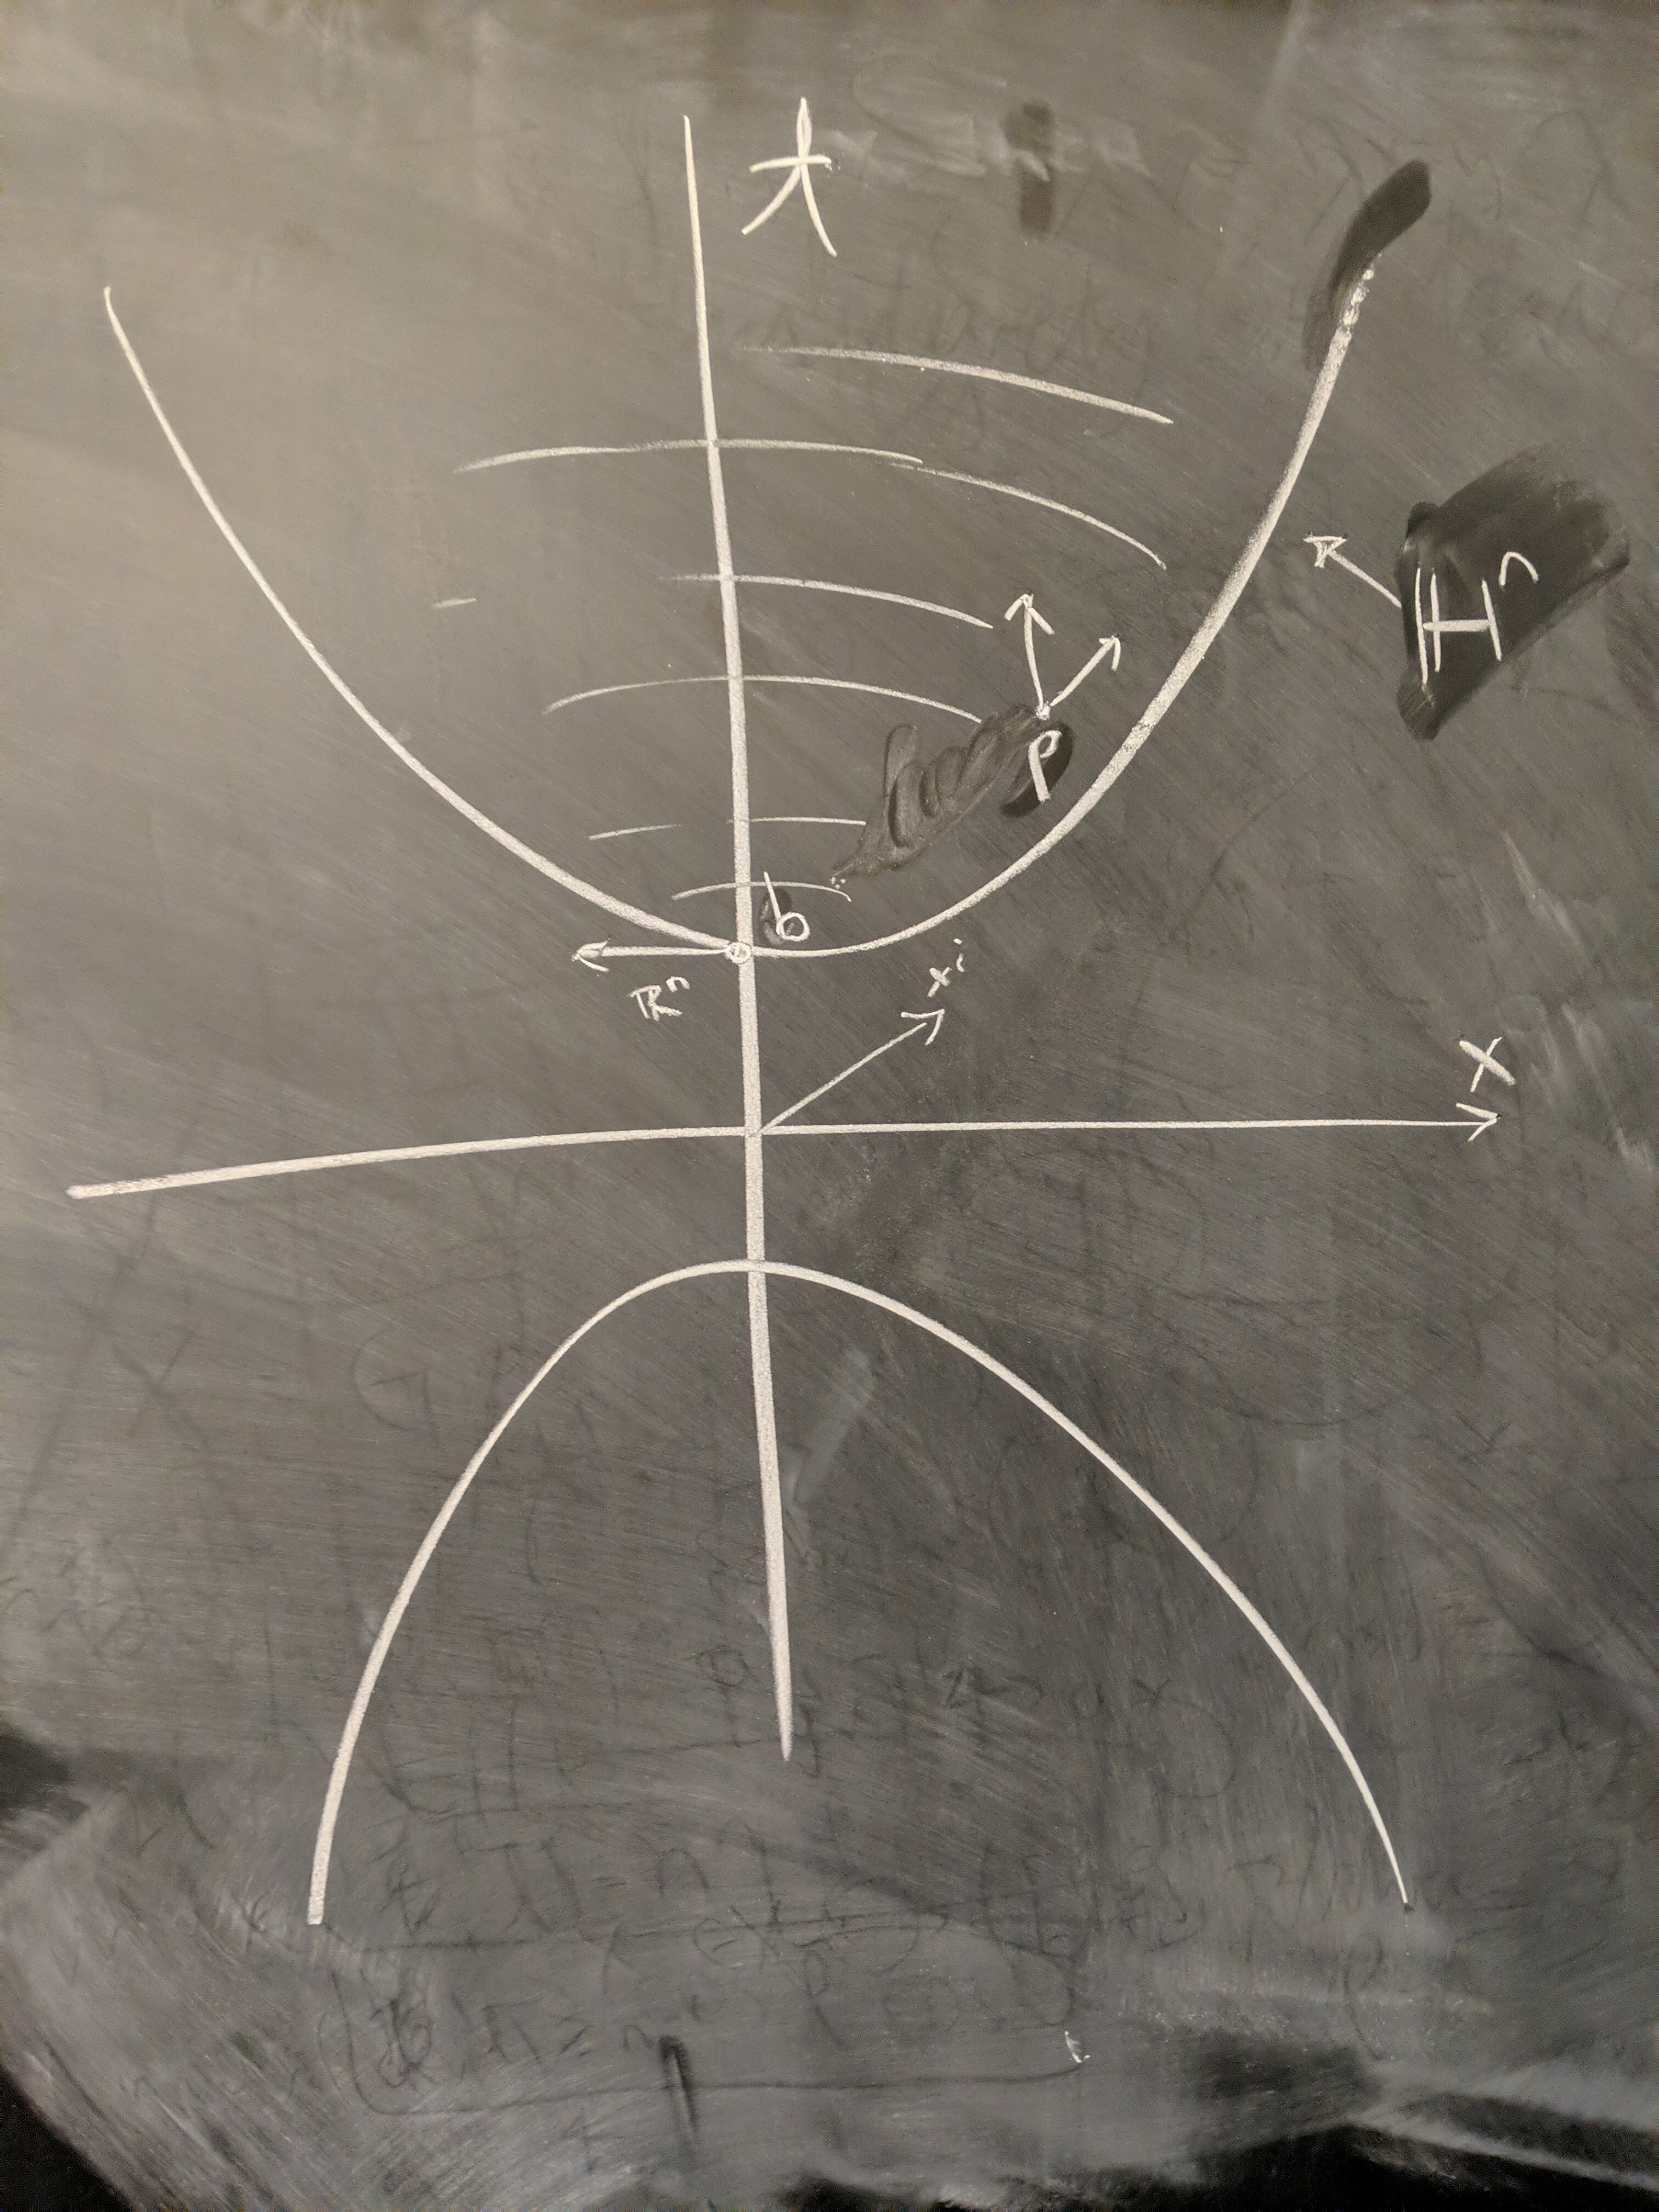
\includegraphics[width=0.3\linewidth]{figures/rgeo_lec5.1.jpg}
\label{hyp} 
\caption{A model of hyperbolic space in $\R^{n+1}$.} 
\end{figure}

For example, at the base $b$ the tangent vectors have no $t$ component, so the inner product is just the one on $\R^n $. The set of isometries are going to be the set of linear isometries of $\R^{n+1}$ with this funny metric $\mathrm O(n,1)$, and it's not hard to cook up one that sends $b\to p$. So the metric on $T_p\H^n $ behaves like the metric on $T_b \H^n $, because the map that sends $b\to q$ preserves the $(n,1)$ inner product, and once you end up at the base $b$ the time coordinate doesn't affect you at all.

So this defines a space where the points all look alike, since $\mathrm O(n,1)$ sends every point to every other point. We need to explicitly construct an element of $\mathrm O(n,1)$ that sends $b \to q$. Let us do this in two dimensions. Say $p$ is of the form $(p,t)=(p^1,0,0,\cdots,t)$. Consider \[
\mleft(\begin{array}{cccccc|c}
    \cosh(\alpha )& & & & & & \sinh(\alpha ) \\
    & 1 & & & & & \\
    & & 1&  & & & \\
    & & & 1 & & & \\
    & & &  & 1& & \\
    & & &  & & 1& \\
    \hline
    \sinh(\alpha )&  & &  & & & \cosh(\alpha )
\end{array}\mright).
\] The claim is that this is an element of $\mathrm O(n,1)$, sending  $(0,0,\cdots ,1)$ to $(\sinh\alpha ,0,0,\cdots ,\cosh\alpha )$. Since $\cosh^2(\alpha )-\sinh^2(\alpha )=1$, there exists an $\alpha $ such that for $(p^1,0,0,\cdots ,t) $, $p^1=\sinh(\alpha )$ and $t=\cosh(\alpha )$ (since $t^2-(x^1)^2=1$ by the definition of our pseudometric). More explicitly, this is the map \[
\mleft(\begin{array}{cccccc|c}
    t& & & & & & x \\
    & 1 & & & & & \\
    & & 1&  & & & \\
    & & & 1 & & & \\
    & & &  & 1& & \\
    & & &  & & 1& \\
    \hline
    x&  & &  & & & t
\end{array}\mright), \quad \text{since} \ t^2-x^2=1.
\] This is an explicit map in $\mathrm O(n,1)$ sending $(0,0,\cdots ,1)\to (x,0,\cdots ,t)$. In $n$ dimensions, replace the component $(x,0,0,\cdots )$ with any vector of length $n$. This gives us our isometries, since if we have an isometry of the underlying vector space $\R^{n+1}$, this induces an isometry on the unit sphere. This unit sphere is actually a \textbf{Riemannian} metric since we have an isometry taking a point with a positive definite metric to another point. So for hyperbolic space,
\[
G=\mathrm O(n,1)=\left\{ A \in M(n+1)\ \left| \
A^T
\begin{pmatrix}
    1 & & &  &0\\
     &1 & &  &\\
     & & 1&  &\\
     & & &1  &\\
     0& & &  &-1 \\
\end{pmatrix}A=
\begin{pmatrix}
    1 & & &  &\\
     &1 & &  &\\
     & & 1&  &\\
     & & &1  &\\
     & & & & -1 \\
\end{pmatrix}
\right. 
 \right\} \] If we replaced the $-1$ factor with 1, this would become the set of matrices $A$ such that $A^TA=I$, which is just $O(n+1)$. Similarly, \[
 H=O(n)=
 \left\{ \left.     \mleft(\begin{array}{ccc|c}
                    & & &  \\
                    & B & &0 \\
                    & & &  \\
                    \hline
                    & 0 & &  1
     \end{array}\mright) \ \right| \ B^TB=I \right\} < O(n+1,1).
 \] So hyperbolic space is frame isotropic! This is the abstract definition of hyperbolic space, but what does the metric look like? We need to get coordinates on $\H^n $, for which there will be several different models. There are three ways:
 \begin{enumerate}[label=(\arabic*)]
     \item Consider the plane $t=1$. For each point $(x,t)$, project down to the origin through that plane. This intersects $t=1$ at a point $x /t$ contained in the unit disk, since $t^2-|x^2|=1$. So $x /t<1$ since $t$ is bigger than $x$.

\begin{figure}[H]
\centering
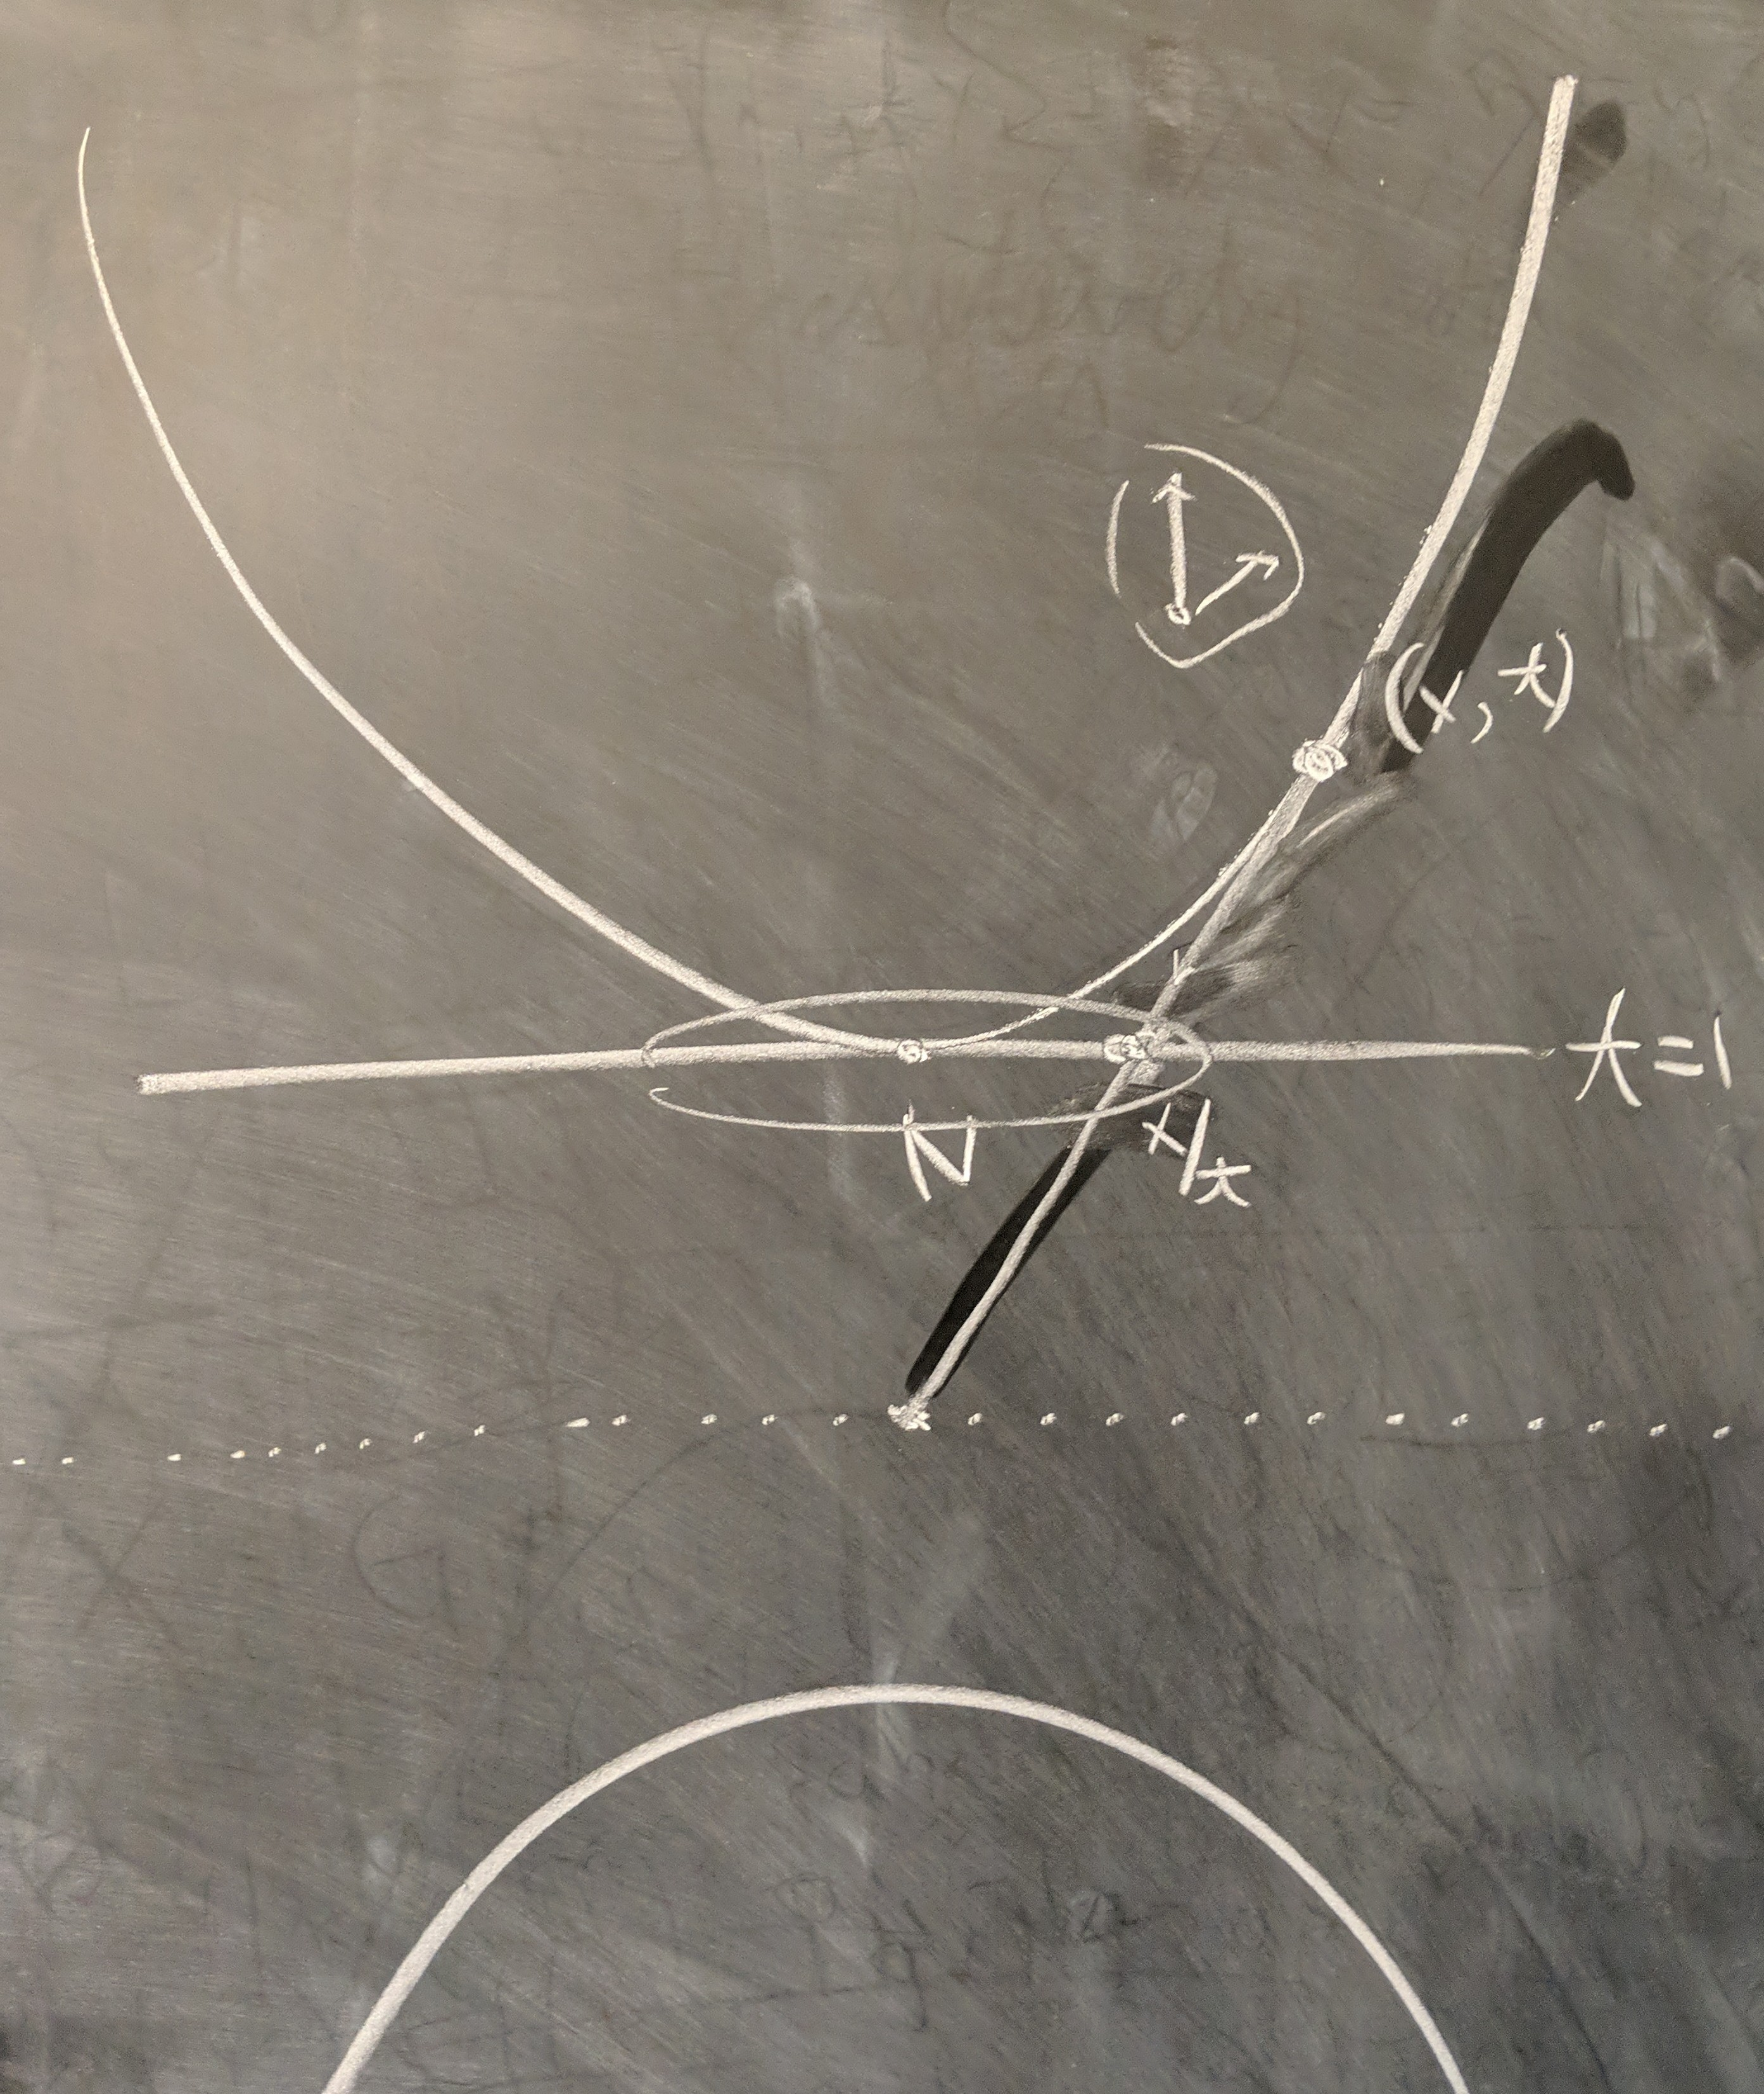
\includegraphics[width=0.4\linewidth]{figures/rgeo_lec5.2.jpg}
\end{figure}

         Parametrizing by points in the unit disk by projection gives us the \textbf{Beltrami-Klein} model.
     \item The second way is by the analogue of stereographic projection. Rather than consider a line through the north pole, we consider a line through $(x,t)$ and the \emph{south pole} $S=(0,-1)$. 

\begin{figure}[H]
\centering
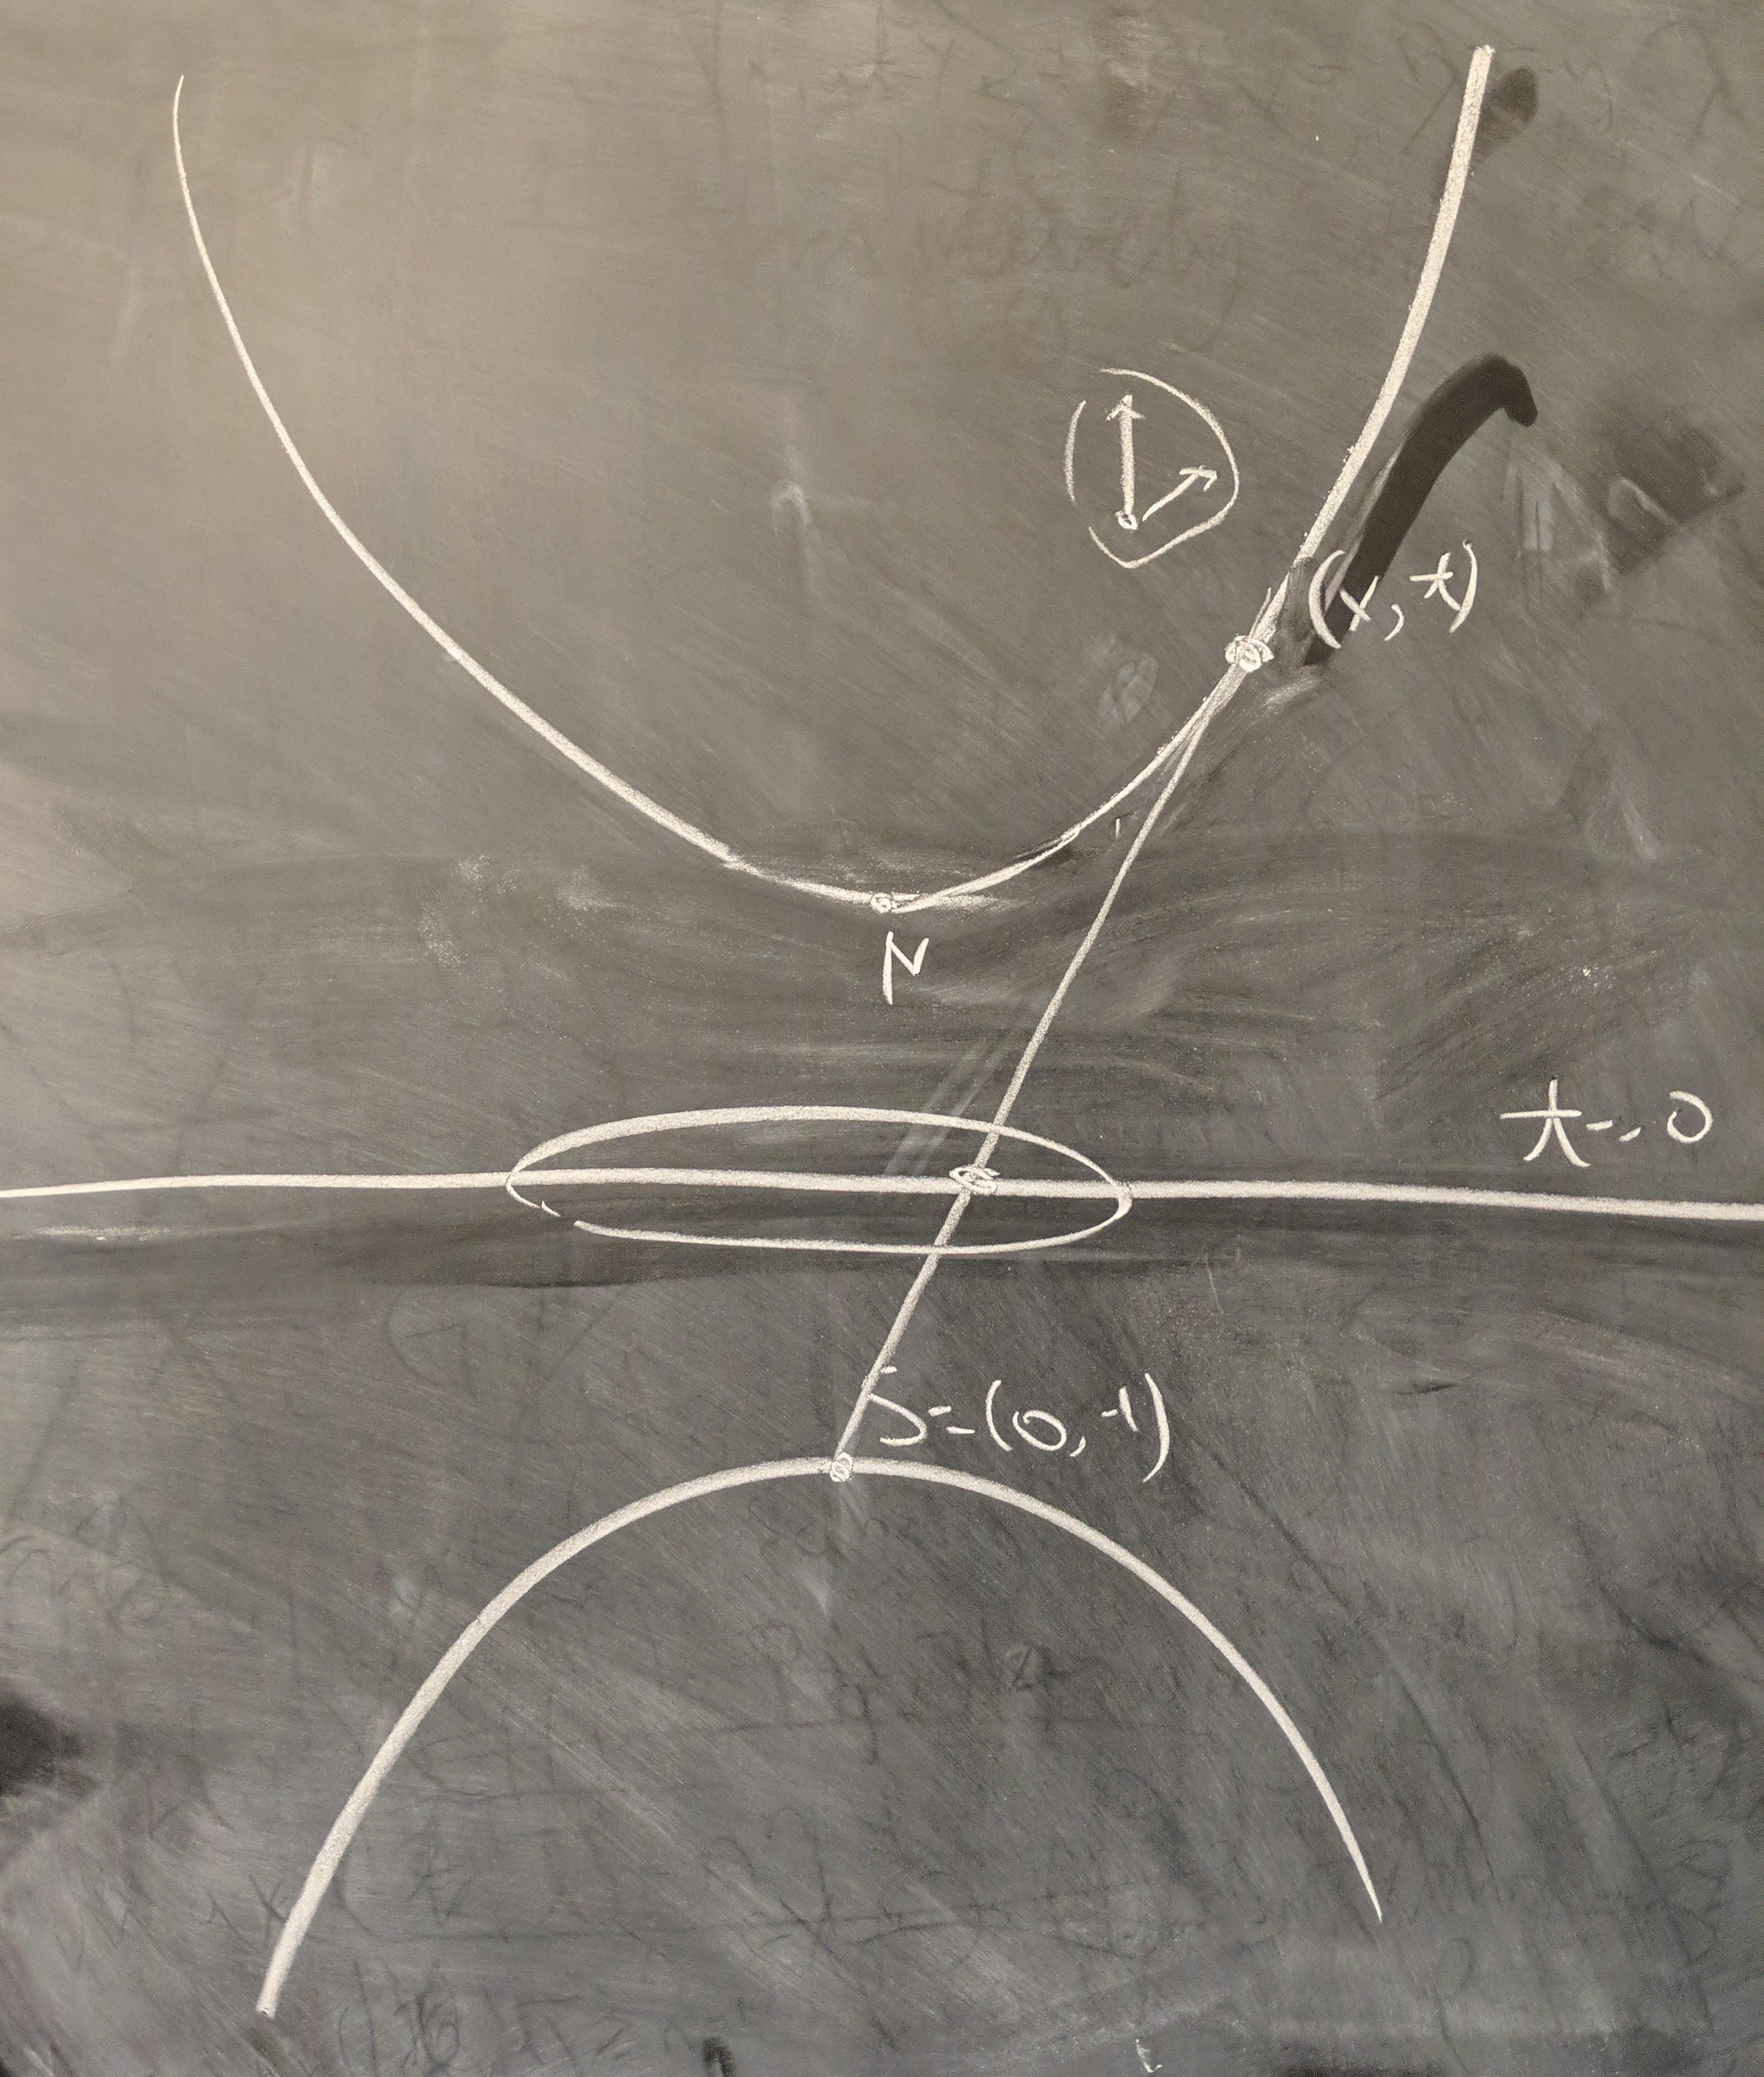
\includegraphics[width=0.4\linewidth]{figures/rgeo_lec5.3.jpg}
\end{figure}

         The point ends up in a unit disk here too, but a different one: in the previous model, we had the Beltrami-Klein disk, while this is called the \textbf{Poincare disk model}. Both will give you metrics (but it turns out this metric will be conformal).
     \item The final model will give us a metric on the \textbf{upper half space}, where we take $\R^{n-1}\times [0,\infty)$ and map the disk onto it.
 \end{enumerate}
 For all of these, first we work it out in two dimensions, then $n$ dimensions. However, we actually understand $n$ dimensional hyperbolic space abstractly: we have seen that $\H^n =\mathrm O(n,1)/\mathrm O(n) $ and is frame isotropic. What is this mysterious frame isotropic space that is not a sphere nor a plane? We will see next time.
